\documentclass[conference]{IEEEtran}
\IEEEoverridecommandlockouts

\usepackage[T1]{fontenc}
\usepackage{amsmath,amssymb}
\usepackage{graphicx}
\usepackage{booktabs}
\usepackage{multirow}
\usepackage{xcolor}
\usepackage[caption=false,font=footnotesize]{subfig}
\usepackage{tikz}
\usetikzlibrary{arrows.meta,positioning,fit}
\usepackage{cite}
\usepackage[hidelinks]{hyperref}

\graphicspath{{../figures/}}
\definecolor{closed}{HTML}{2A78D6}
\definecolor{open}{HTML}{EB6834}
\definecolor{ink2}{HTML}{52514E}
\newcommand{\vect}[1]{\mathbf{#1}}

\begin{document}

\title{Closing the Loop on Jenga: Visual Servoing and\\Force Sensing for Block Extraction in Simulation}

\author{
\IEEEauthorblockN{Somanshu Juneja, Dharmesh Sahu, and Pramukto Mandal}
\IEEEauthorblockA{Indian Institute of Technology Mandi, Himachal Pradesh, India}
}

\maketitle

\begin{abstract}
Pushing a block out of a Jenga tower needs the fingertip within a few millimetres
of the block's centre, and a decision, made by touch, about whether the block is
free to move. We rebuild a low-cost Jenga-playing pipeline in PyBullet, around a
7-DOF Franka Panda with an eye-in-hand RGB-D camera and a one-axis fingertip force
sensor: block-face detection, a two-sub-space selection policy, inverse kinematics
with trapezoidal motion, 2\textonehalf-D visual servoing, and a force-thresholded
push. The simulation includes the error sources that make the real task hard:
block tolerances, robot calibration error and depth-sensor bias. Over 18 paired
towers per setup, closed-loop servoing aligns the finger to $0.14$\,mm (ground-truth
detection) and $0.90$\,mm (a classical OpenCV detector) and scores $15.7$ and $15.3$
successful attempts per game. Open-loop positioning from the same estimates misses by
$3$--$4.5$\,mm on average, pushes the wrong block in a quarter of its attempts and scores
$10.3$ and $10.9$. A force threshold applied over the first 15\,mm of travel separates
mobile from immobile blocks without a learned model. Code and data are public.
\end{abstract}

\begin{IEEEkeywords}
Jenga, visual servoing, eye-in-hand camera, force sensing, manipulation, PyBullet
\end{IEEEkeywords}

% ---------------------------------------------------------------------------
\section{Introduction}

Jenga compresses several hard manipulation problems into one game. A robot must
find each block, choose one that is safe to remove, bring a fingertip to the
centre of a $25\times15$\,mm face, and push the block out without toppling a
tower that grows less stable after every move. Two properties make it a useful
benchmark. First, precision: with an 11\,mm wide fingertip, the contact point must
lie within about 7\,mm of the face centre or the finger catches a neighbour. Second,
vision alone cannot tell whether a block is free. Friction between blocks depends on
manufacturing tolerances and on earlier moves, so the robot has to feel the block
before committing to the push.

Marchionna \emph{et al.}~\cite{marchionna2023} showed that a cost-effective arm, a
depth camera and a cheap one-axis force sensor are enough to play, scoring up to 14
consecutive extractions. Their system detects blocks with a deep instance-segmentation
network, tracks the target with a model-based tracker, aligns the fingertip by
visual servoing and classifies the block with a force threshold during the push.

We rebuild that pipeline in simulation and use the controlled setting to answer a
question that is costly to study on hardware: \emph{how much does closing the loop
with vision matter, and how good must the detector be?} We contribute:
\begin{itemize}
\item a complete, open PyBullet implementation of the four-stage pipeline on a
7-DOF Panda, with a simulated spring-loaded force sensor and an eye-in-hand RGB-D
camera;
\item an error model (block tolerances, joint-encoder bias, depth noise and scale
error) without which simulation makes open-loop control look perfect;
\item a paired comparison of closed- and open-loop control with ground-truth and
classical OpenCV detection over 72 full games, using the success metric of
\cite{marchionna2023}.
\end{itemize}

% ---------------------------------------------------------------------------
\section{Related Work}

Kr\"oger \emph{et al.}~\cite{kroger2008} played Jenga with an industrial manipulator,
a laser scanner and a force/torque sensor, reaching 29 extractions in a simplified
setting. Kimura \emph{et al.}~\cite{kimura2010} modelled the forces acting on a pushed
block and used a six-axis sensor to decide removability, achieving 14 consecutive
extractions. Wang \emph{et al.}~\cite{wang2009} used only vision and inexpensive
hardware and reached 5 on a simplified, half-height tower. Fazeli
\emph{et al.}~\cite{fazeli2019} learned a hierarchical model from vision and touch and
reached 20. Bauza \emph{et al.}~\cite{bauza2017} trained a deep Q-network in simulation
to push a block without a model of the tower. Ziglar~\cite{ziglar2006}
analysed the static mechanics of the tower and the friction that holds a loaded
block in place.

Visual servoing~\cite{hutchinson1996,chaumette2006} closes the loop between image
measurements and robot motion. Position-based schemes regulate an estimated pose;
image-based schemes regulate image features. The 2\textonehalf-D scheme of Malis
\emph{et al.}~\cite{malis1999} mixes the two, combining image coordinates of a point,
the logarithm of its depth ratio and the rotation error, and is the scheme used in
\cite{marchionna2023} through ViSP~\cite{marchand2005}.

% ---------------------------------------------------------------------------
\section{System}

\begin{figure}[t]
\centering
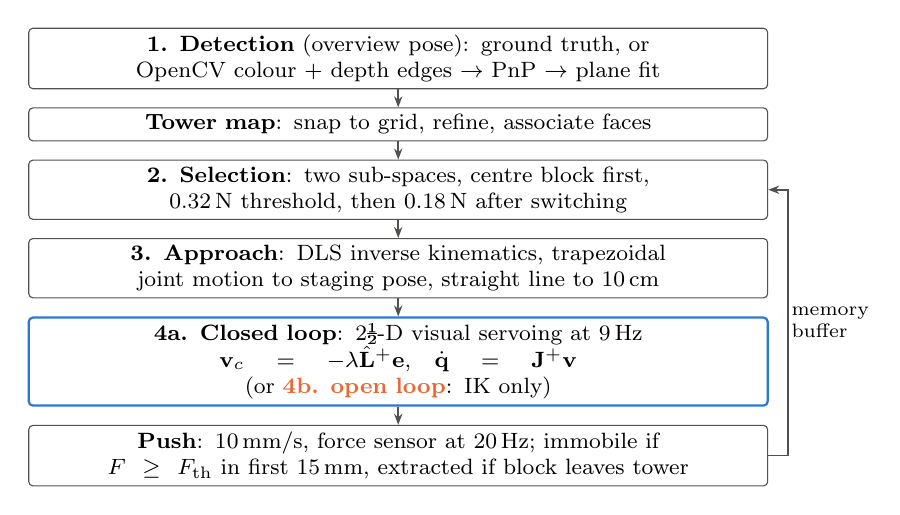
\begin{tikzpicture}[
  node distance=2.3mm,
  box/.style={draw=ink2, rounded corners=1.5pt, align=center, font=\footnotesize,
              text width=0.76\columnwidth, inner sep=2.4pt, fill=white},
  arr/.style={-{Stealth[length=4pt]}, draw=ink2, line width=0.6pt}]
\node[box] (det) {\textbf{1. Detection} (overview pose): ground truth, or\\
  OpenCV colour + depth edges $\rightarrow$ PnP $\rightarrow$ plane fit};
\node[box, below=of det] (map) {\textbf{Tower map}: snap to grid, refine, associate faces};
\node[box, below=of map] (pol) {\textbf{2. Selection}: two sub-spaces, centre block first,\\
  0.32\,N threshold, then 0.18\,N after switching};
\node[box, below=of pol] (ik) {\textbf{3. Approach}: DLS inverse kinematics, trapezoidal\\
  joint motion to staging pose, straight line to 10\,cm};
\node[box, below=of ik, draw=closed, line width=0.8pt] (vs) {\textbf{4a. Closed loop}: 2\textonehalf-D visual servoing at 9\,Hz\\
  $\vect{v}_c=-\lambda\hat{\vect{L}}^{+}\vect{e}$,\quad $\dot{\vect{q}}=\vect{J}^{+}\vect{v}$\\
  (or \textcolor{open}{\textbf{4b. open loop}}: IK only)};
\node[box, below=of vs] (push) {\textbf{Push}: 10\,mm/s, force sensor at 20\,Hz; immobile if\\
  $F\ge F_{\text{th}}$ in first 15\,mm, extracted if block leaves tower};
\foreach \a/\b in {det/map, map/pol, pol/ik, ik/vs, vs/push} \draw[arr] (\a) -- (\b);
\draw[arr] (push.east) -- ++(2.5mm,0) |- node[pos=0.25, right, font=\scriptsize, align=left, inner sep=1pt]{memory\\buffer} (pol.east);
\end{tikzpicture}
\caption{The pipeline for one attempt. The outcome updates the policy's memory of each
block before the next overview.}
\label{fig:pipeline}
\end{figure}

\begin{figure*}[t]
\centering
\subfloat[Overview image with OpenCV face estimates]{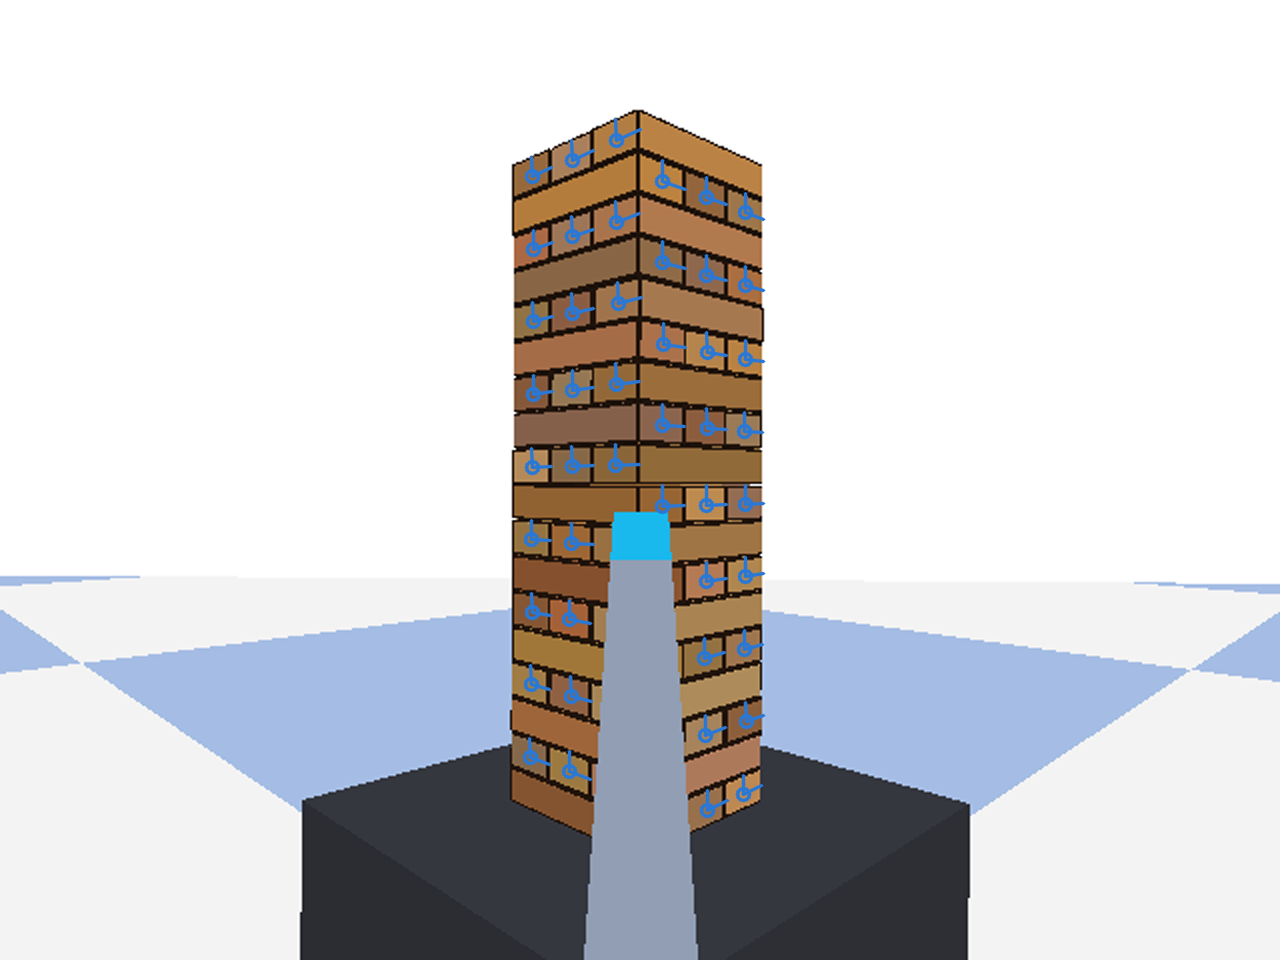
\includegraphics[width=0.315\textwidth]{camera_overview.png}\label{fig:scene:overview}}\hfill
\subfloat[Close-up after servoing; target in red]{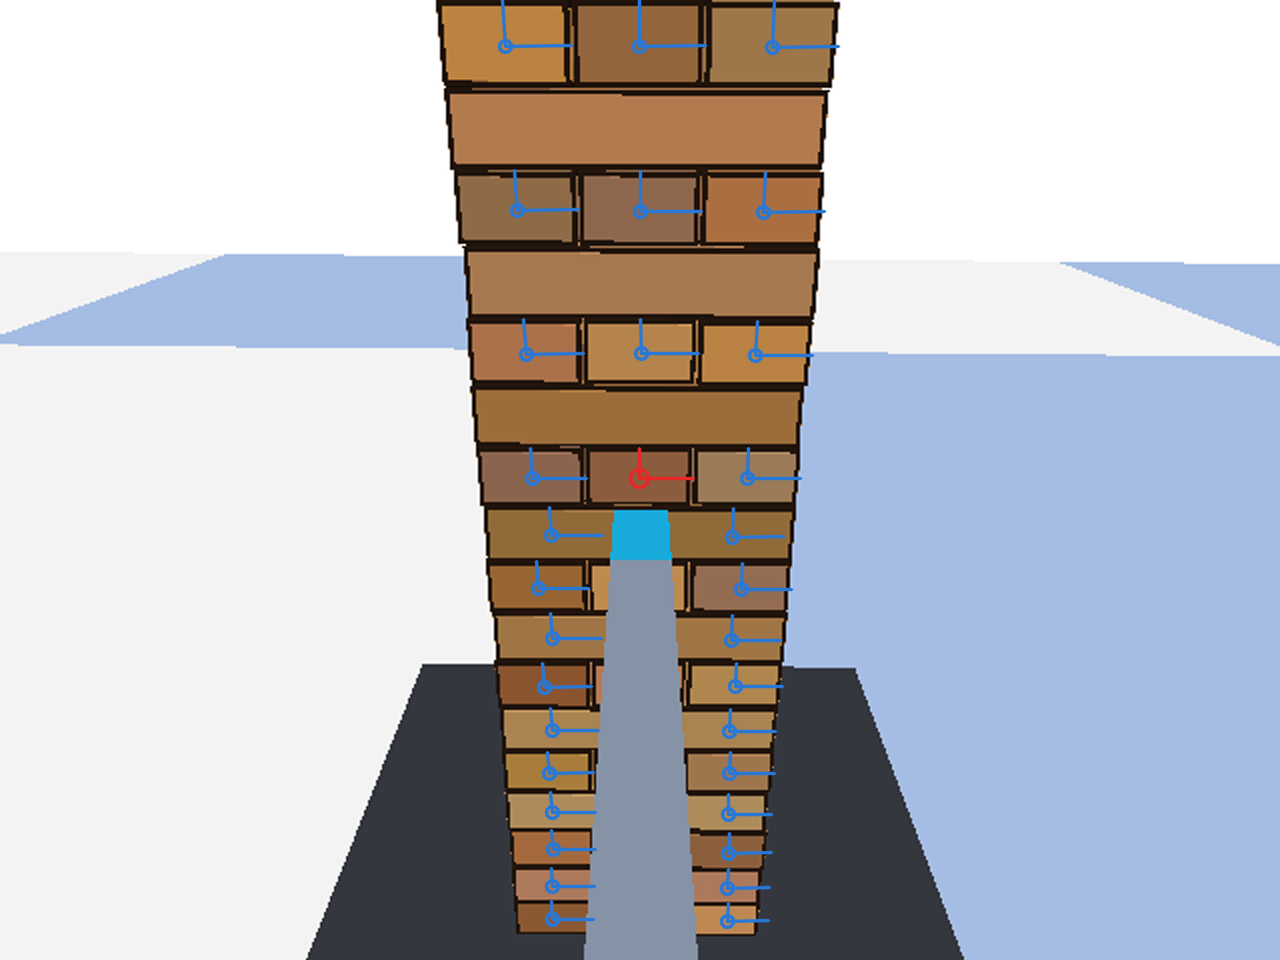
\includegraphics[width=0.315\textwidth]{camera_aligned.png}\label{fig:scene:aligned}}\hfill
\subfloat[A level-10 block halfway out]{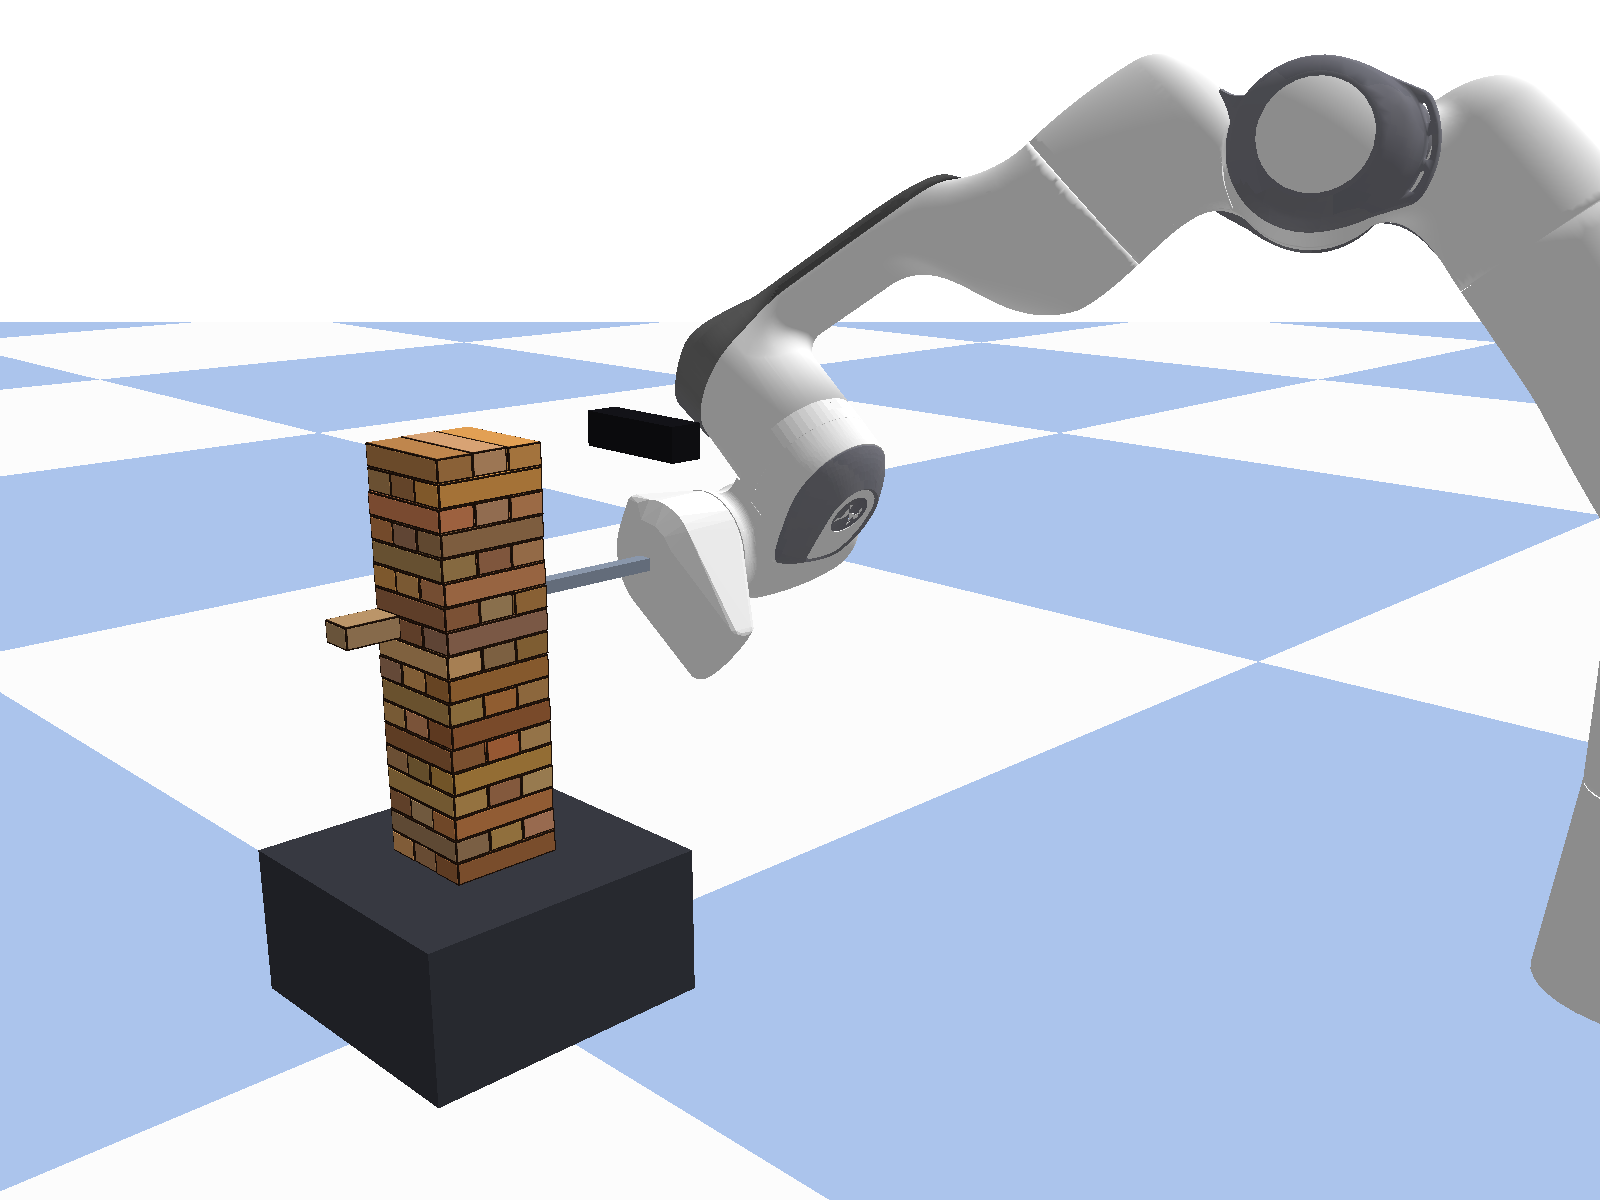
\includegraphics[width=0.315\textwidth]{scene_push_side.png}\label{fig:scene:push}}
\caption{The simulated system. (a)~From the overview pose the eye-in-hand camera sees two
faces of the tower; each circle is a detected face centre and the short lines are its
estimated horizontal and vertical axes. (b)~At the end of servoing the target face (red)
sits where the camera expects it when the fingertip (cyan, bottom centre) is 25\,mm in
front of the face centre. (c)~External view during a push.}
\label{fig:scene}
\end{figure*}

\subsection{Simulation}

The scene (Fig.~\ref{fig:scene}) holds an 18-level, 54-block tower on a 10\,cm
stand and a Franka Panda, simulated in PyBullet~\cite{coumans2016}, whose hand is replaced by a 170\,mm finger with an
$11\times9$\,mm tip. Blocks measure $75\times25\times15$\,mm, weigh 19.6\,g and have
friction coefficient $\mu=0.4$~\cite{ziglar2006}. Physics runs at 240\,Hz with 300
solver iterations; fewer iterations under-resolve friction in a tall stack and make
every block look mobile. Resting blocks use anchored friction and are allowed to sleep,
which removes the slow creep of stacked boxes in Bullet.

The force sensor is modelled physically: the fingertip is a 20\,g body on a prismatic
joint with a 100\,N/m spring, so its reading comes from the simulated contact and only
measures force along the finger. Readings are tared before each push, sampled at
20\,Hz and quantised to 12 bits over 5\,N. The camera (640$\times$480, 60$^\circ$
field of view) sits 80\,mm above and 150\,mm behind the fingertip, pitched to look at
the face the finger is about to touch.

\textbf{Error model.} A noiseless simulator makes open-loop control trivially
accurate, so we model three error sources (Table~\ref{tab:params}). Each block's
height varies with $\sigma=0.1$\,mm and its position by up to $\pm0.5$\,mm, so towers
differ in where they bind. Each joint encoder has a fixed offset ($\sigma=0.17^\circ$):
the controller's kinematic model, inverse kinematics and camera pose are slightly
wrong, while images are always rendered from the true camera pose. The depth image
has per-pixel noise of $0.5(1+z^2)$\,mm and a per-camera scale error ($\sigma=1\%$).

\begin{table}[t]
\centering
\caption{Simulation and controller parameters}
\label{tab:params}
\footnotesize
\setlength{\tabcolsep}{4pt}
\begin{tabular}{@{}ll@{}}
\toprule
Block size, mass, friction $\mu$ & $75{\times}25{\times}15$\,mm, 19.6\,g, 0.4 \\
Block height tolerance, jitter & $\sigma=0.1$\,mm, $\pm0.5$\,mm \\
Joint-encoder offset & $\sigma=0.003$\,rad per joint \\
Depth noise, depth scale error & $0.5(1+z^2)$\,mm, $\sigma=1\%$ \\
Physics rate, solver iterations & 240\,Hz, 300 \\
Servo rate, gain $\lambda$ & 9\,Hz, 1.5 \\
Servo stop (lateral, axial, angle) & 0.5\,mm, 1\,mm, 0.005\,rad \\
Servo timeout, tracking loss & 15\,s, 5 missed frames \\
Sensor stiffness, rate, resolution & 100\,N/m, 20\,Hz, 12\,bit over 5\,N \\
Push speed, classification travel & 10\,mm/s, 15\,mm \\
Force thresholds (sub-space 1, 2) & 0.32\,N, 0.18\,N \\
Safety limit after 15\,mm & 0.64\,N \\
\bottomrule
\end{tabular}
\end{table}

\subsection{Detection}

From an overview pose 30\,cm from the tower's corner the camera sees both pushable
faces (Fig.~\ref{fig:scene:overview}). The \emph{ground-truth} detector takes face
poses from the simulator for every block whose face centre is visible in the
segmentation mask. It is an upper bound on perception, not a cheat on the rest of the
pipeline: the observed pose is still mapped to the world through the robot's
(biased) kinematic model.

The \emph{OpenCV} detector never reads simulator poses. It thresholds the image in HSV
to keep wood colour, removes pixels on strong depth gradients so touching faces
separate, and labels connected components. For each component it estimates a pose
with planar PnP (IPPE~\cite{collins2014}) on the minimum-area rectangle, refines it
with a plane fit to the component's depth points, and rejects components whose size
does not match an end face. This replaces the deep segmentation network
of~\cite{marchionna2023} with a classical baseline.

\textbf{Tower map.} Detections are associated with blocks through a nominal
layer/slot grid. Calibration error shifts every detected face by several millimetres,
and differently at each arm pose, so the grid is registered from each image before
association: a coarse step snaps detections to the nearest layer of matching
orientation (layers of one orientation repeat every 30\,mm, so a shift of up to
$\pm15$\,mm is unambiguous) and the nearest slot, and a fine step takes the median
in-plane residual per axis. Depth along the face normal is ignored because it
legitimately varies, for example for half-pushed blocks.

\subsection{Block selection}

The policy follows~\cite{marchionna2023}. Levels 2--15 are split into two sub-spaces,
levels 2--8 and 9--15; the bottom two and top two levels are never pushed. The game
starts in a random sub-space with a 0.32\,N threshold; once every level there has been
tested it switches to the other sub-space and a more cautious 0.18\,N, since the tower
is weaker by then. Within a level the centre block is tried first; after an immobile
block the rest of the level is tried, and at most one block is extracted per level.
A memory buffer stores each block's status. An attempt that ends in an error is
retried once, then the block is skipped. A game ends when the tower collapses, when
no candidate is left, or after 60 attempts.

\subsection{Approach}

Inverse kinematics is solved with damped least squares on the controller's model,
\begin{equation}
\Delta\vect{q} = \vect{J}^{\top}\big(\vect{J}\vect{J}^{\top}+\mu^{2}\vect{I}\big)^{-1}\vect{e}
 + \big(\vect{I}-\vect{J}^{+}\vect{J}\big)\,k\,(\vect{q}_{\text{mid}}-\vect{q}),
\end{equation}
from several seeds, keeping joint limits and preferring the solution closest to the
current configuration. The second term uses the Panda's redundancy to stay near
mid-range. The arm moves to a staging pose 20\,cm in front of the target face with a
trapezoidal joint-space profile, then in a straight line to 10\,cm.

\subsection{Alignment by visual servoing}

From 10\,cm the closed-loop controller regulates the pose of the target face in the
camera frame towards the pose it has when the fingertip is 25\,mm in front of the face
centre and parallel to its normal. With the face centre at normalised image
coordinates $(x,y)$ and depth $Z$, the feature error is
\begin{equation}
\vect{e} = \big(x-x^{*},\; y-y^{*},\; \log(Z/Z^{*}),\; \theta\vect{u}\big),
\end{equation}
where $\theta\vect{u}$ is the axis-angle rotation between the current and desired
camera frames~\cite{malis1999}. The camera twist is
\begin{equation}
\vect{v}_c = -\lambda\,\hat{\vect{L}}^{+}\vect{e},\qquad
\hat{\vect{L}} =
\begin{bmatrix}
\vect{L}_{v} & \vect{L}_{\omega}\\
\vect{0} & \vect{I}_3
\end{bmatrix},
\end{equation}
with $\vect{L}_v,\vect{L}_\omega$ the translational and rotational rows of the
point-and-depth interaction matrix. The twist is clipped to 4\,cm/s and 0.4\,rad/s,
transformed to the tool frame and mapped to joints by resolved-rate control,
\begin{equation}
\dot{\vect{q}} = \vect{J}^{+}_{\text{DLS}}\,\vect{v} + \big(\vect{I}-\vect{J}^{+}\vect{J}\big)\,k\,(\vect{q}_0-\vect{q}),
\end{equation}
with a posture term that holds the null-space motion near the configuration at the
start of servoing. Images arrive at 9\,Hz; between them the commanded joint velocity
is held at the physics rate.

The servo locks onto its target in the first close-up frame by registering the tower
map from that image and picking the face associated with the target's level and slot;
it then follows the nearest detection within 12\,mm. Comparing world positions
directly across the overview and close-up poses fails, because the two calibration
errors differ by up to 12\,mm. The \emph{open-loop} baseline skips servoing: it moves
straight to the 25\,mm clearance pose computed from the overview estimate.

\subsection{Push and classification}

The push runs open loop at 10\,mm/s along the finger axis while the sensor is read at
20\,Hz. The force threshold is a classification test: it applies until the block has
moved 15\,mm, which proves it mobile. After that a 0.64\,N safety limit applies
instead, because near the end of an extraction the block tips against the level above
and friction rises (Fig.~\ref{fig:forces}, left); applying the threshold all the way
would stop pushes on blocks that are almost out. A block counts as extracted once it
has moved one block length plus 1\,mm, or if it tips out of the tower before the
finger finishes. An immobile call counts as correct only if the finger was touching
the target alone; a force measured through another block is an error.

% ---------------------------------------------------------------------------
\section{Experiments}

We compare four setups, the product of two detectors (ground truth, OpenCV) and two
controllers (closed loop, open loop). Each runs 18 games, the number of trials
in~\cite{marchionna2023}, and game $i$ uses the same random seed in all four setups:
the same block tolerances, friction pattern and calibration error. Results are
therefore paired by tower.

Following~\cite{marchionna2023}, an attempt is \emph{successful} if the block is
extracted, or correctly classified as immobile, without collapsing the tower. The
primary metric is the number of successful attempts per game. The tower counts as
collapsed if any block other than the target drops by half a block height, tilts more
than $20^\circ$, or slides half a block length. Errors are unreachable poses, lost
tracking, servo timeouts, pushes on the wrong block, and pushes that do not clear the
block (for example, a side block that yaws off the finger). Alignment error is the
distance from the fingertip axis to the true face centre at the start of the push.
Intervals are 95\,\% Student-$t$ intervals over games.

% ---------------------------------------------------------------------------
\section{Results}

\begin{table*}[t]
\centering
\caption{Results over 18 games per setup (mean $\pm$ 95\,\% interval over games; maxima in brackets)}
\label{tab:main}
\footnotesize
\setlength{\tabcolsep}{5pt}
\begin{tabular}{@{}llcccccccc@{}}
\toprule
Controller & Detector & Attempts & Successful / game & Extractions / game & Extracted & Immobile & Error & Collapse & Alignment error \\
\midrule
\multirow{2}{*}{Closed loop} & Ground truth & 307 & $\mathbf{15.7\pm4.4}$ [27] & $5.7\pm1.7$ [12] & 33.2\,\% & 58.6\,\% & 4.2\,\% & 3.9\,\% & $0.14\pm0.07$\,mm \\
 & OpenCV & 294 & $\mathbf{15.3\pm4.3}$ [29] & $5.6\pm1.8$ [13] & 34.0\,\% & 59.5\,\% & 2.4\,\% & 4.1\,\% & $0.90\pm0.35$\,mm \\
\midrule
\multirow{2}{*}{Open loop} & Ground truth & 280 & $10.3\pm4.1$ [31] & $3.8\pm1.5$ [11] & 24.6\,\% & 41.4\,\% & 27.9\,\% & 6.1\,\% & $3.12\pm2.53$\,mm \\
 & OpenCV & 297 & $10.9\pm4.0$ [27] & $3.4\pm1.5$ [12] & 20.5\,\% & 45.5\,\% & 28.6\,\% & 5.4\,\% & $4.52\pm4.82$\,mm \\
\bottomrule
\end{tabular}

\vspace{2pt}
{\footnotesize Alignment error is mean $\pm$ standard deviation over attempts. Outcome
shares are of all attempts; an attempt during which the tower collapsed counts only
as a collapse.}
\end{table*}

\begin{figure}[t]
\centering
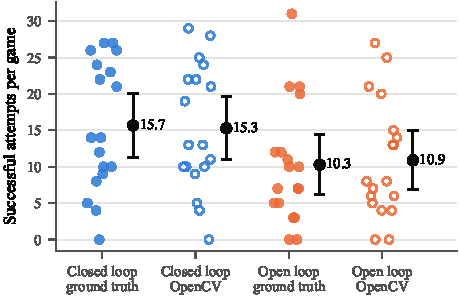
\includegraphics[width=\columnwidth]{successes.pdf}
\caption{Successful attempts per game. Each dot is one game (filled: ground-truth
detection; hollow: OpenCV); black marks show the mean and 95\,\% interval. Colour
marks the controller (blue: closed loop; orange: open loop).}
\label{fig:successes}
\end{figure}

\subsection{Closed versus open loop}

Table~\ref{tab:main} and Fig.~\ref{fig:successes} summarise the 72 games. Closing the
loop raises the number of successful attempts per game by about half, from 10.3 to
15.7 with ground-truth detection and from 10.9 to 15.3 with OpenCV. Because games are
paired by tower, we test the difference per tower. With ground-truth detection the
closed loop wins on 13 towers, loses on 2 and ties on 3 (mean difference $+5.4$,
paired $t_{17}=3.14$, $p=0.006$; sign test $p=0.007$). With OpenCV it wins on 13 and
loses on 3 ($+4.4$, $t_{17}=1.80$, $p=0.09$; sign test $p=0.02$). The spread between
towers is large: the same seed tends to give a long or a short game in every setup,
which is why the paired tests are more informative than the overlapping intervals.

The mechanism is alignment (Fig.~\ref{fig:alignment}). Servoing brings the finger to
within 0.5\,mm of the face centre with ground-truth detection and within 2.3\,mm with
OpenCV, in every attempt. Open-loop positioning from the same overview estimates has
a median error of 2.2\,mm (ground truth) and 3.7\,mm (OpenCV), and 10--15\,\% of
attempts exceed the 7\,mm tolerance. Those misses become errors: 144 of the 163
open-loop errors are pushes in which the finger pressed on a neighbouring block, so
the force it measured did not belong to the target. The closed loop never made this
error.

Open-loop errors are not spread evenly. They concentrate on the odd levels, whose
faces point along $-y$ (Fig.~\ref{fig:levels}, right: up to 54\,\% of attempts at
level 15), while even levels see almost none. The two face orientations need
different arm configurations, and the same joint offsets map to different fingertip
errors in each; with these offsets the $-y$ configurations put the finger outside the
tolerance more often. The closed loop removes this dependence because it measures the
face relative to the camera at the pose where it pushes.

\begin{figure*}[t]
\centering
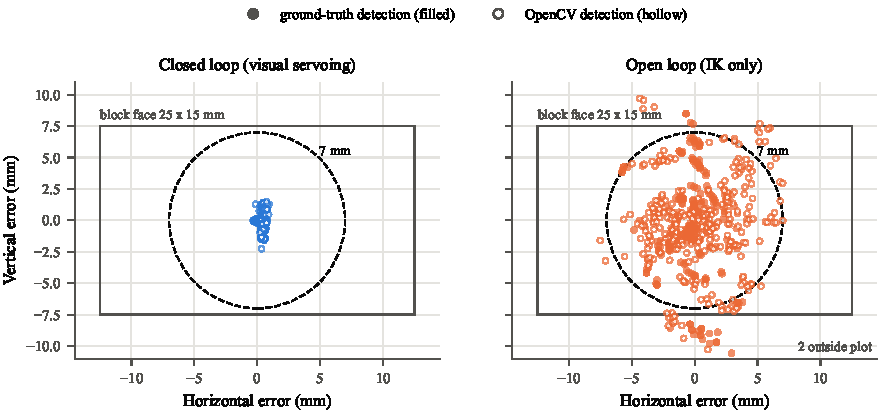
\includegraphics[width=0.9\textwidth]{alignment.pdf}
\caption{Contact point relative to the face centre at the start of each push, for all
attempts that reached the push. The dashed circle is the 7\,mm tolerance and the
rectangle is the face. Two open-loop OpenCV attempts fall outside the plotted area.}
\label{fig:alignment}
\end{figure*}

\subsection{Effect of the detector}

With the closed loop, the classical detector costs almost nothing: 15.3 against 15.7
successful attempts per game (paired difference $+0.4$, $p=0.86$). OpenCV's 0.9\,mm
alignment error is mostly vertical ($\sigma_v=0.80$\,mm against $\sigma_h=0.13$\,mm):
the 15\,mm face height spans few pixels at the close-up distance, and the dark seams
at the top and bottom of a face likely bias its estimated centre. Both are far inside the tolerance.
This agrees with the argument in~\cite{marchionna2023} that the servo loop, not the
detector's absolute accuracy, is what makes precise pushing possible: the detector
only has to be consistent from frame to frame.

The detector matters more for open-loop control, whose OpenCV alignment error has a
heavier tail (95th percentile 8.7\,mm, maximum 56\,mm). Ground-truth detection does not rescue the open loop either, because the
error that dominates there is calibration, not perception.

\subsection{Force-based classification}

\begin{figure*}[t]
\centering
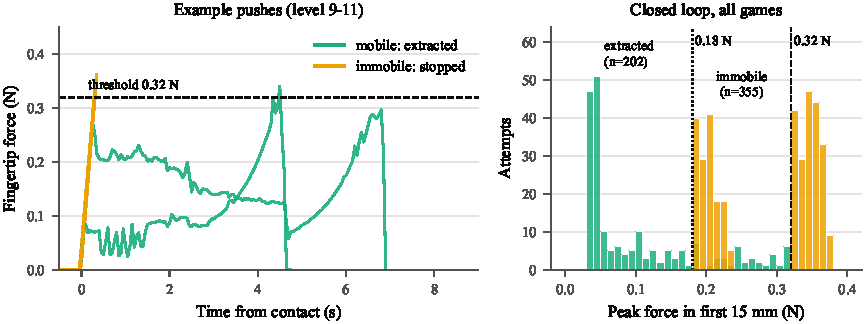
\includegraphics[width=0.9\textwidth]{forces.pdf}
\caption{Left: fingertip force in eight consecutive pushes of one game (levels 9--11).
Immobile blocks reach the threshold within 0.4\,s of contact; mobile blocks slide at
0.05--0.25\,N and show a late rise when they tip against the level above, after the
15\,mm classification window. Right: peak force inside the window for all closed-loop
pushes. Immobile peaks sit just above the threshold of their phase.}
\label{fig:forces}
\end{figure*}

Fig.~\ref{fig:forces} shows the force signal behind each decision. In the first
sub-space the peak force inside the classification window averaged
$0.114\pm0.093$\,N for blocks that came out and $0.345\pm0.015$\,N for immobile blocks;
in the second, $0.075\pm0.044$\,N and $0.201\pm0.014$\,N. Immobile peaks sit slightly
above their threshold because the sensor is sampled at 20\,Hz while the force rises
quickly against a stuck block. The friction rise at the end of an extraction often
exceeds 0.32\,N (left panel), which is why the threshold must stop applying once the
block has proved mobile; applied throughout, it would stop such pushes before the
block cleared the tower.

Fig.~\ref{fig:levels} shows where blocks came free. Under the closed loop, 10--31\,\%
of attempts on levels 2--8 extracted a block, against 33--61\,\% on levels 9--15. Lower
blocks carry more of the tower's weight, so more of them bind; this is the
load-dependent friction that~\cite{ziglar2006} describes and the reason vision alone
cannot judge removability. Collapses concentrate near the top (7 of 30 closed-loop
attempts on level 15), where little weight holds the remaining blocks in place.

\begin{figure*}[t]
\centering
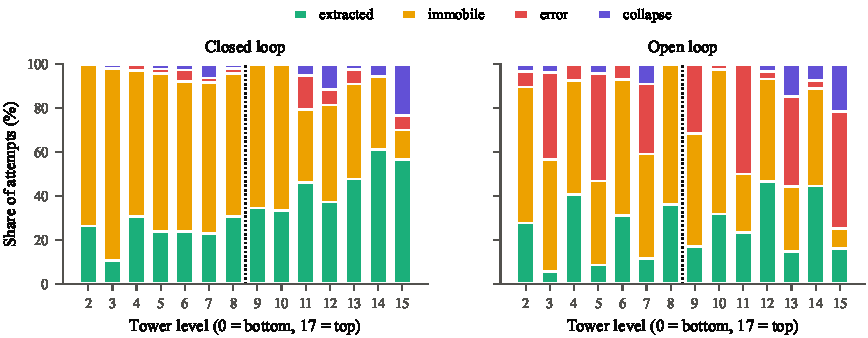
\includegraphics[width=0.9\textwidth]{levels.pdf}
\caption{Outcome by tower level, pooled over both detectors. The dotted line separates
the two sub-spaces. Open-loop errors concentrate on odd levels, whose faces point
along $-y$.}
\label{fig:levels}
\end{figure*}

\subsection{Servoing time and failure modes}

Servoing converged in $3.43\pm0.34$\,s (about 30 visual updates) with ground-truth
detection and $3.50\pm0.22$\,s with OpenCV, roughly constant across levels, as
in~\cite{marchionna2023}. Closed-loop errors were rare: 13 pushes that did not clear the
block, mostly side blocks that yawed off the finger, and 7 attempts in which the
ground-truth detector lost the target because a block left half-pushed by an earlier
attempt hid it from the camera. Twelve of the 18 closed-loop games in each detector
setup ended in a collapse; the rest ended when no candidate block was left.

\subsection{Comparison with the physical system}

\begin{table}[t]
\centering
\caption{Comparison with the physical system of~\cite{marchionna2023}}
\label{tab:physical}
\footnotesize
\setlength{\tabcolsep}{4pt}
\begin{tabular}{@{}lccc@{}}
\toprule
 & Physical & \multicolumn{2}{c}{Simulated, closed loop} \\
\cmidrule(l){3-4}
 & \cite{marchionna2023} & Ground truth & OpenCV \\
\midrule
Successful attempts / game & 13.8 & 15.7 & 15.3 \\
Extractions / game & 7.5 & 5.7 & 5.6 \\
Share of attempts successful & 80\,\% & 92\,\% & 94\,\% \\
Extracted/immobile/error (\%) & 45/35/20 & 33/59/8 & 34/60/6 \\
Most extractions in a game & 14 & 12 & 13 \\
Alignment error & $<0.2$\,mm mean & 0.14\,mm & 0.90\,mm \\
\bottomrule
\end{tabular}

\vspace{2pt}
{\footnotesize Simulated error shares include collapses.}
\end{table}

Table~\ref{tab:physical} places the closed-loop results next to the physical system.
Successful attempts per game and the maximum number of extractions are similar. The
simulated robot makes fewer errors, because it has no lighting changes, no
segmentation failures and no singular configurations at the edge of the workspace,
which caused most errors on hardware. It also finds more immobile blocks and extracts
fewer. Two differences explain this: the physical game placed extracted blocks back
on top, adding load and new levels to play, and Bullet's iterative solver
under-resolves friction in a tall stack, so the simulated forces fall in the right
0--1\,N range but are not calibrated Coulomb values.

% ---------------------------------------------------------------------------
\section{Limitations}

These are simulation results. Friction forces are approximate, as noted above, and
the block mass and friction come from the literature rather than a measured set.
Extracted blocks are removed rather than stacked on top, and the tower is never moved
between sub-spaces; the Panda reaches every level from one base position. The OpenCV
detector stands in for a trained segmentation network and benefits from rendered
seams between faces, and per-frame detection with data association replaces a
model-based tracker. Finally, the error model is a choice: larger calibration error
would widen the gap between the controllers, and a real depth camera has structured
errors that the noise model does not capture.

% ---------------------------------------------------------------------------
\section{Conclusion}

A simulated Panda with an eye-in-hand camera and a one-axis force sensor plays Jenga
at a level comparable to the physical system it is modelled on, and the controlled
setting isolates where that performance comes from. Visual servoing is the key
component: it keeps alignment under a millimetre and adds about five successful
attempts per game over open-loop positioning on the same towers. With the loop
closed, a classical detector performs as well as perfect perception. A force threshold
applied only while the block starts to move is enough to classify removability.

A natural next step is to replace the rule-based selection policy with a learned one
that maximises the length of a game, in the spirit of~\cite{bauza2017,fazeli2019},
using this simulation to generate experience. Code, data and figure scripts are
available at \url{https://github.com/tomoeOOseven/jenga-robot-simulation}.

% ---------------------------------------------------------------------------
\begin{thebibliography}{99}

\bibitem{marchionna2023}
L.~Marchionna, G.~Pugliese, M.~Martini, S.~Angarano, F.~Salvetti, and M.~Chiaberge,
``Deep instance segmentation and visual servoing to play Jenga with a cost-effective
robotic system,'' \emph{arXiv:2211.07977}, 2023.

\bibitem{kroger2008}
T.~Kr\"oger, B.~Finkemeyer, S.~Winkelbach, L.-O. Eble, S.~Molkenstruck, and F.~M. Wahl,
``A manipulator plays Jenga,'' \emph{IEEE Robot. Autom. Mag.}, vol.~15, no.~3,
pp.~79--84, 2008.

\bibitem{kimura2010}
S.~Kimura, T.~Watanabe, and Y.~Aiyama, ``Force based manipulation of Jenga blocks,''
in \emph{Proc. IEEE/RSJ Int. Conf. Intell. Robots Syst. (IROS)}, 2010, pp.~4287--4292.

\bibitem{wang2009}
J.~Wang, P.~Rogers, L.~Parker, D.~Brooks, and M.~Stilman, ``Robot Jenga: Autonomous
and strategic block extraction,'' in \emph{Proc. IEEE/RSJ Int. Conf. Intell. Robots
Syst. (IROS)}, 2009, pp.~5248--5253.

\bibitem{fazeli2019}
N.~Fazeli, M.~Oller, J.~Wu, Z.~Wu, J.~B. Tenenbaum, and A.~Rodriguez, ``See, feel, act:
Hierarchical learning for complex manipulation skills with multisensory fusion,''
\emph{Sci. Robot.}, vol.~4, no.~26, eaav3123, 2019.

\bibitem{bauza2017}
S.~Bauza, J.~Castillo, A.~Nanz, and B.~Kambalur, ``Deep Q-learning applied to a Jenga
playing robot,'' preprint, 2017.

\bibitem{ziglar2006}
J.~Ziglar, ``Analysis of mechanics in Jenga,'' Robotics Institute, Carnegie Mellon
University, 2006.

\bibitem{hutchinson1996}
S.~Hutchinson, G.~D. Hager, and P.~I. Corke, ``A tutorial on visual servo control,''
\emph{IEEE Trans. Robot. Autom.}, vol.~12, no.~5, pp.~651--670, 1996.

\bibitem{chaumette2006}
F.~Chaumette and S.~Hutchinson, ``Visual servo control, Part~I: Basic approaches,''
\emph{IEEE Robot. Autom. Mag.}, vol.~13, no.~4, pp.~82--90, 2006.

\bibitem{malis1999}
E.~Malis, F.~Chaumette, and S.~Boudet, ``2\textonehalf-D visual servoing,''
\emph{IEEE Trans. Robot. Autom.}, vol.~15, no.~2, pp.~238--250, 1999.

\bibitem{marchand2005}
E.~Marchand, F.~Spindler, and F.~Chaumette, ``ViSP for visual servoing: A generic
software platform with a wide class of robot control skills,'' \emph{IEEE Robot.
Autom. Mag.}, vol.~12, no.~4, pp.~40--52, 2005.

\bibitem{collins2014}
T.~Collins and A.~Bartoli, ``Infinitesimal plane-based pose estimation,''
\emph{Int. J. Comput. Vis.}, vol.~109, no.~3, pp.~252--286, 2014.

\bibitem{coumans2016}
E.~Coumans and Y.~Bai, ``PyBullet, a Python module for physics simulation for games,
robotics and machine learning,'' \url{http://pybullet.org}, 2016--2021.

\end{thebibliography}

\end{document}
